\documentclass[tikz,border=12pt]{standalone}
\usepackage[T1]{fontenc}
\usepackage{mathpazo}
\usepackage{amsmath,amssymb}
\usetikzlibrary{arrows.meta, positioning, calc, decorations.pathreplacing}

\definecolor{stblue}{HTML}{7B97AD}
\definecolor{rwgold}{HTML}{B8995E}
\definecolor{sage}{HTML}{7A9A7E}
\definecolor{dkbrown}{HTML}{3D3530}
\definecolor{wmgray}{HTML}{7B7067}
\definecolor{cream}{HTML}{F9F6F0}
\definecolor{border}{HTML}{D4C9B8}
\definecolor{terracotta}{HTML}{C47A6A}

\begin{document}
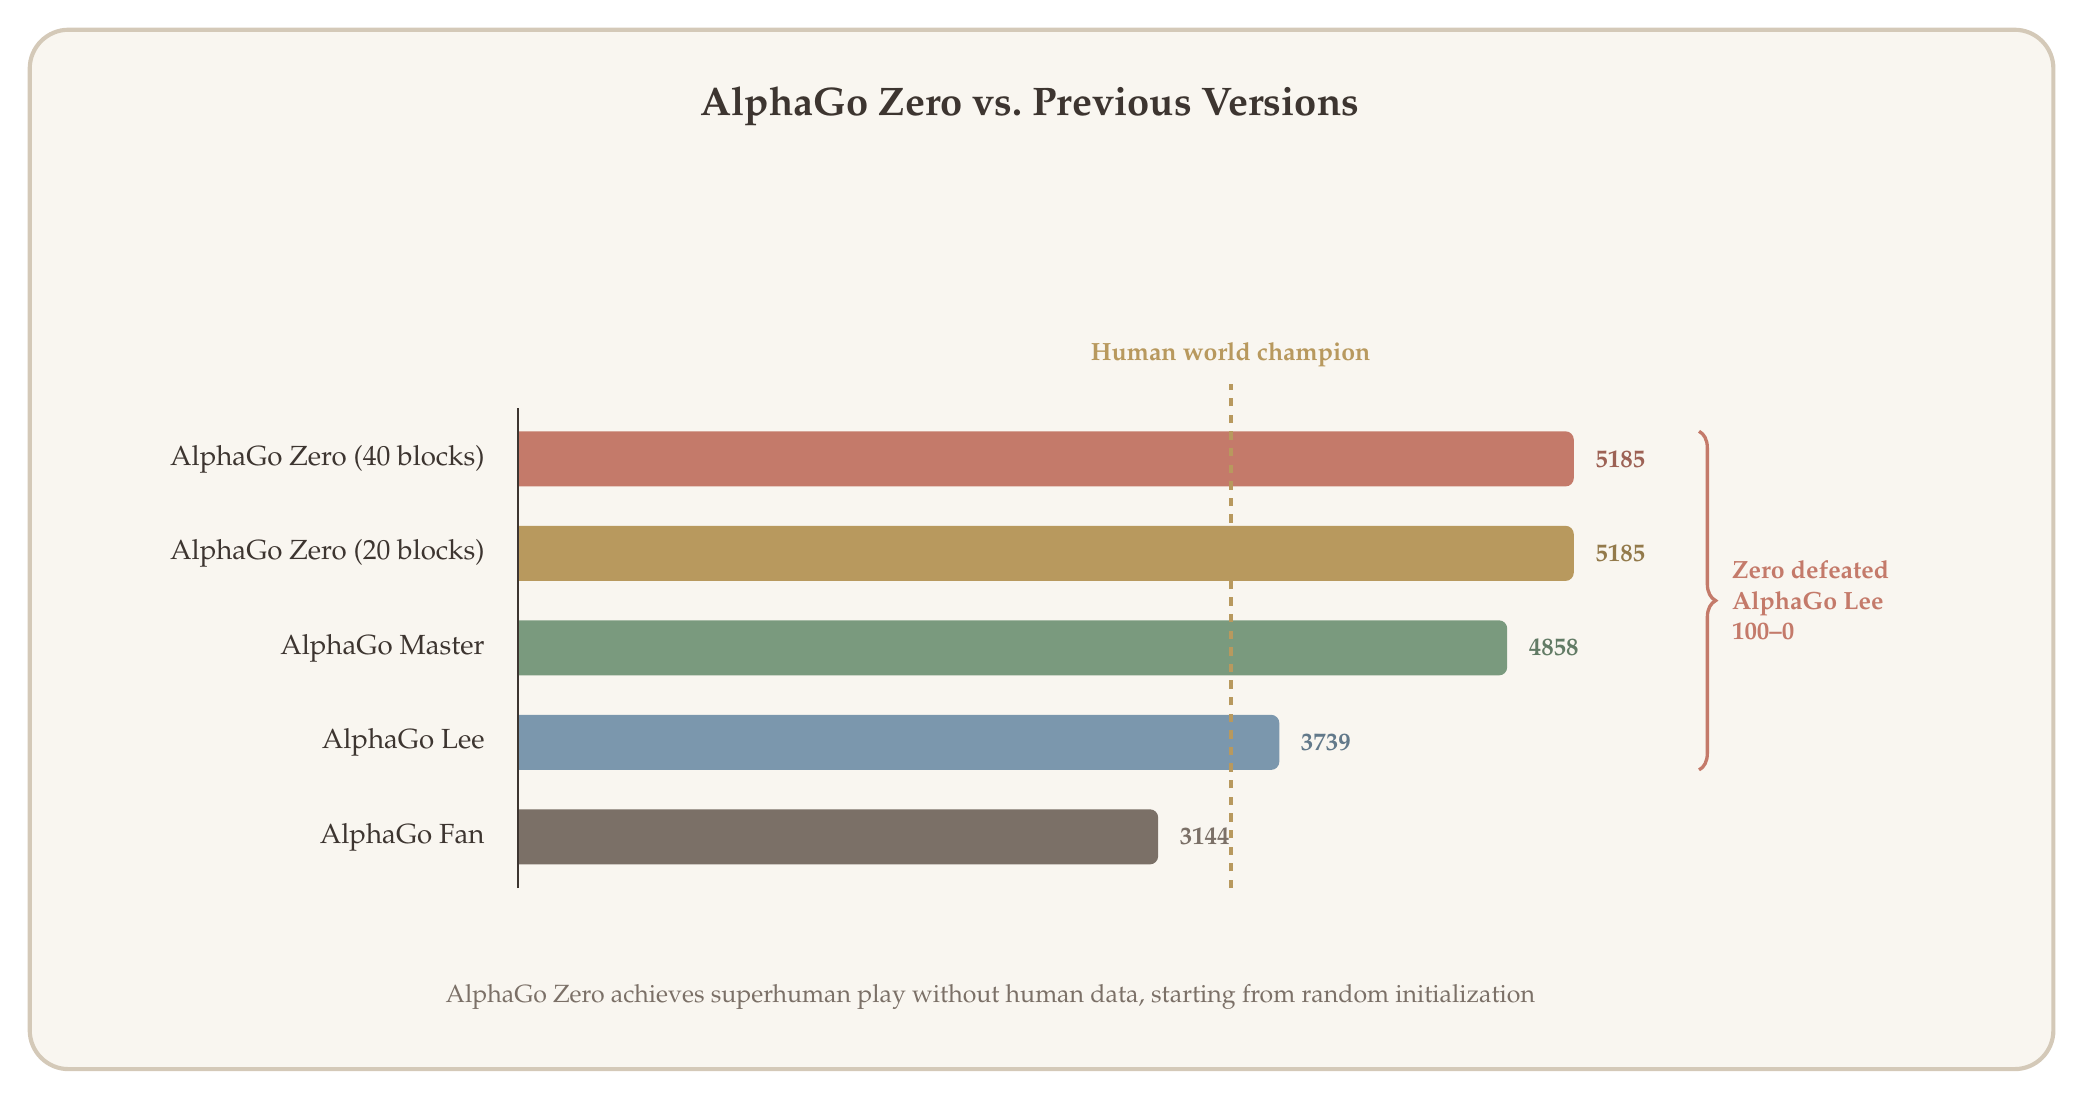
\begin{tikzpicture}[
  >={Stealth[length=3.5mm, width=2.5mm]},
]

% Dimensions
\pgfmathsetmacro{\barh}{0.7}       % bar height
\pgfmathsetmacro{\barstep}{1.2}    % vertical step between bars
\pgfmathsetmacro{\maxelo}{5800}     % x-axis max for scaling
\pgfmathsetmacro{\chartw}{15}       % chart width in cm
\pgfmathsetmacro{\labelx}{-0.3}     % right edge of label text

% Bar base y
\pgfmathsetmacro{\boney}{0.6}

% Background
\fill[cream, rounded corners=14pt] (-6.2,-2) rectangle (19.5,11.2);
\draw[border, rounded corners=14pt, line width=1.5pt] (-6.2,-2) rectangle (19.5,11.2);

% Title
\node[font=\Large\bfseries, text=dkbrown, anchor=north] at (6.5,10.6)
  {AlphaGo Zero vs.\ Previous Versions};

% Data: sorted bottom (lowest) to top (highest)
% Bar 1: AlphaGo Fan    3144  wmgray
% Bar 2: AlphaGo Lee    3739  stblue
% Bar 3: AlphaGo Master 4858  sage
% Bar 4: AlphaGo Zero (20 blocks)  5185  rwgold
% Bar 5: AlphaGo Zero (40 blocks)  5185  terracotta

% --- AlphaGo Fan ---
\pgfmathsetmacro{\yy}{\boney + 0*\barstep}
\pgfmathsetmacro{\bw}{3144/\maxelo*\chartw}
\fill[wmgray, rounded corners=0pt]
  (0,\yy) [rounded corners=3pt] -- (\bw,\yy) -- (\bw,\yy+\barh)
  [rounded corners=0pt] -- (0,\yy+\barh) -- cycle;
\node[font=\normalsize, text=dkbrown, anchor=east] at (\labelx, \yy+\barh/2)
  {AlphaGo Fan};
\node[font=\small\bfseries, text=wmgray, anchor=west] at (\bw+0.15, \yy+\barh/2)
  {3144};

% --- AlphaGo Lee ---
\pgfmathsetmacro{\yy}{\boney + 1*\barstep}
\pgfmathsetmacro{\bw}{3739/\maxelo*\chartw}
\fill[stblue, rounded corners=0pt]
  (0,\yy) [rounded corners=3pt] -- (\bw,\yy) -- (\bw,\yy+\barh)
  [rounded corners=0pt] -- (0,\yy+\barh) -- cycle;
\node[font=\normalsize, text=dkbrown, anchor=east] at (\labelx, \yy+\barh/2)
  {AlphaGo Lee};
\node[font=\small\bfseries, text=stblue!80!black, anchor=west] at (\bw+0.15, \yy+\barh/2)
  {3739};

% --- AlphaGo Master ---
\pgfmathsetmacro{\yy}{\boney + 2*\barstep}
\pgfmathsetmacro{\bw}{4858/\maxelo*\chartw}
\fill[sage, rounded corners=0pt]
  (0,\yy) [rounded corners=3pt] -- (\bw,\yy) -- (\bw,\yy+\barh)
  [rounded corners=0pt] -- (0,\yy+\barh) -- cycle;
\node[font=\normalsize, text=dkbrown, anchor=east] at (\labelx, \yy+\barh/2)
  {AlphaGo Master};
\node[font=\small\bfseries, text=sage!80!black, anchor=west] at (\bw+0.15, \yy+\barh/2)
  {4858};

% --- AlphaGo Zero (20 blocks) ---
\pgfmathsetmacro{\yy}{\boney + 3*\barstep}
\pgfmathsetmacro{\bw}{5185/\maxelo*\chartw}
\fill[rwgold, rounded corners=0pt]
  (0,\yy) [rounded corners=3pt] -- (\bw,\yy) -- (\bw,\yy+\barh)
  [rounded corners=0pt] -- (0,\yy+\barh) -- cycle;
\node[font=\normalsize, text=dkbrown, anchor=east] at (\labelx, \yy+\barh/2)
  {AlphaGo Zero (20 blocks)};
\node[font=\small\bfseries, text=rwgold!80!black, anchor=west] at (\bw+0.15, \yy+\barh/2)
  {5185};

% --- AlphaGo Zero (40 blocks) ---
\pgfmathsetmacro{\yy}{\boney + 4*\barstep}
\pgfmathsetmacro{\bw}{5185/\maxelo*\chartw}
\fill[terracotta, rounded corners=0pt]
  (0,\yy) [rounded corners=3pt] -- (\bw,\yy) -- (\bw,\yy+\barh)
  [rounded corners=0pt] -- (0,\yy+\barh) -- cycle;
\node[font=\normalsize, text=dkbrown, anchor=east] at (\labelx, \yy+\barh/2)
  {AlphaGo Zero (40 blocks)};
\node[font=\small\bfseries, text=terracotta!80!black, anchor=west] at (\bw+0.15, \yy+\barh/2)
  {5185};

% --- Vertical baseline at x=0 ---
\draw[dkbrown, line width=0.8pt] (0,0.3) -- (0,\boney + 4*\barstep + \barh + 0.3);

% --- Human world champion dashed line at Elo 3500 ---
\pgfmathsetmacro{\profx}{3500/\maxelo*\chartw}
\draw[rwgold, line width=1.5pt, dashed]
  (\profx,0.3) -- (\profx,\boney + 4*\barstep + \barh + 0.6);
\node[font=\small\bfseries, text=rwgold, anchor=south]
  at (\profx, \boney + 4*\barstep + \barh + 0.7)
  {Human world champion};

% --- Annotation brace: Zero defeated AlphaGo Lee 100-0 ---
% Brace on the right spanning AlphaGo Lee to AlphaGo Zero (40 blocks)
\pgfmathsetmacro{\leey}{\boney + 1*\barstep}
\pgfmathsetmacro{\zeroy}{\boney + 4*\barstep + \barh}
\pgfmathsetmacro{\bracex}{15}
\draw[decorate, decoration={brace, amplitude=6pt}, line width=1.2pt, terracotta]
  (\bracex, \zeroy) -- (\bracex, \leey)
  node[midway, right, xshift=8pt, font=\small\bfseries, text=terracotta, align=left]
  {Zero defeated\\AlphaGo Lee\\100--0};

% --- Bottom annotation ---
\node[font=\small, text=wmgray, anchor=north, align=center] at (6,-0.8)
  {AlphaGo Zero achieves superhuman play without human data,
   starting from random initialization};

\end{tikzpicture}
\end{document}
